\documentclass[12pt]{report}

%%%%%%%%%%%%%%%%%%%%%%%%%%%%%%%%%%%%%%%%%%%%%%%%%%%%%%%%

%%% General Packages
\usepackage{amsmath, amssymb, amsthm}
\usepackage{titling}
\usepackage{titlesec}
\usepackage{geometry}
\usepackage{enumerate}

\usepackage[hidelinks]{hyperref}



%%% Font and Text Packages
\usepackage{newpxtext}
\usepackage{newpxmath}

\usepackage[dvipsnames]{xcolor}


%%% Graphics, Figure and Listing Packages
\usepackage{graphicx}
\usepackage{float}
\usepackage{calc}
\usepackage{caption}
\usepackage{subcaption}


%%% Listings
\usepackage{listings}
\usepackage{lstfiracode}


%%% Bibliography Packages
\usepackage[style=alphabetic]{biblatex}
\bibliography{references}

%%%%%%%%%%%%%%%%%%%%%%%%%%%%%%%%%%%%%%%%%%%%%%%%%%%%%%%%

%%% Page Formatting Options
\geometry{left = 2.5cm}
\geometry{right = 2.5cm}
\geometry{top = 2.5cm}
\geometry{bottom = 2.5cm}

%%% Section and Chapter Titling Options
\titleformat{\chapter}[block]
  {\normalfont\Large\bfseries}{Chapter \thechapter}{1em}{\Large}
\titlespacing*{\chapter}{0pt}{40pt}{30pt}
\titleformat*{\section}{\large\bfseries}

%%% Hyperlink Formatting Options
\hypersetup{
    colorlinks,
    linkcolor={black},
    citecolor={blue!60!black},
    urlcolor={blue!80!black}
}

%%%%%%%%%%%%%%%%%%%%%%%%%%%%%%%%%%%%%%%%%%%%%%%%%%%%%%%%

%%% Graphics and Figure Options
% Graphics path (necessary for .svg images).
\graphicspath{{graphics/}}
\counterwithout{figure}{chapter}

% Caption setup
\captionsetup{margin=1.5cm}


%%% Listings Options
\definecolor{codegreen}{rgb}{0,0.6,0}
\definecolor{codegray}{rgb}{0.5,0.5,0.5}
\definecolor{codepurple}{rgb}{0.58,0,0.82}
\definecolor{codeback}{rgb}{0.95,0.95,0.92}
\lstset{
	language=Python,
	backgroundcolor=\color{codeback},   
	commentstyle=\color{codegreen},
	keywordstyle=\color{magenta},
	numberstyle=\tiny\color{codegray},
	style=FiraCodeStyle,   % Use predefined FiraCodeStyle
	basicstyle=\ttfamily,   % Use \ttfamily for source code listings
	numbers=left
}

%%%%%%%%%%%%%%%%%%%%%%%%%%%%%%%%%%%%%%%%%%%%%%%%%%%%%%%%

%%% Personal Macros
\newcommand{\N}{\mathbb{N}}
\newcommand{\R}{\mathbb{R}}
\newcommand{\Z}{\mathbb{Z}}
\renewcommand{\S}{\mathbb{S}}
\newcommand{\ip}[2]{\langle #1, #2 \rangle}

%%% Drafting Macros
\newcommand{\notered}[1]{{\color{Red} \textbf{#1}}}
\newcommand{\notegreen}[1]{{\color{Green} \textbf{#1}}}
\newcommand{\noteblue}[1]{{\color{Blue} \textbf{#1}}}

%%% Theorem Options
\newtheorem*{theorem}{Theorem}
\newtheorem*{proposition}{Proposition}


%%%%%%%%%%%%%%%%%%%%%%%%%%%%%%%%%%%%%%%%%%%%%%%%%%%%%%%%

\begin{document}
	
%%% Make titlepage.

% Titlepage Options
\author{Damian Lin}
\title{Virtualising the $d$-invariant}

\cleardoublepage \thispagestyle{empty}
\null \vfil
\begingroup
\LARGE \bfseries \centering
\openup \medskipamount
\thetitle \par \vspace{30pt}
\centering \mdseries \theauthor \par \bigskip
\endgroup
\vfil \vfil \vfil
\begin{center}
	An essay submitted in partial fulfilment of\\
	the requirements for the degree of\\
	Bachelor of Science/Bachelor of Advanced Studies (Honours)
	\vfil\vfil
	{\large Pure Mathematics\\[5pt]
		University of Sydney}\\
	\vskip6mm
	
\includegraphics[width=25mm]{graphics/USY_MB1_CMYK_Stacked_Logo}
	\vfil
	\normalsize\today
\end{center}
\vfil
\cleardoublepage

\tableofcontents

\chapter*{Introduction}
\addcontentsline{toc}{chapter}{Introduction}

\notegreen{Introduction...}

\notered{very draft}
In order to keep this text relatively self-contained, we begin in Chapter 1 with the study of knots, for without the bread and butter of knot theory, knot invariants. This provides some motivation for the rest of this chapter in which we slowly build our way up to a a specific invariant, the lattice of integer flows, closely following the work of Greene \cite{lattices-graphs-mutation}. We then look at the formulation given by Greene, the $d$-invariant and how that relates to Heegard-Floer homology and another formulation of the $d$-invariant. In Chapter 2, we examine virtual knots, a generalisation of knots with a multitude of equivalent formulations that allows knots to have diagrams on an orientable surface of any genus. The aim of this is to extend the lattice of integer flows to the virtual setting, and examine what properties it is able maintain in this new environment. We suspect the virtual $d$-invariant is less powerful than another invariant known as the Gordon-Litherland Linking Form, and we examine their relationship in Chapter $3$ with the hope in chapter $4$ of finding an example to prove this. In Chapter $5$ we examine an algorithm to compute these invariants, and present a proof that indeed, the virtual $d$-invariant is not as strong as the Gordon-Litherland Linking Form, and therefore not a complete mutation invariant of alternating knots.

\chapter{Knots and the Lattice of Integer Flows}

\section{Knots and Knot Invariants}

We begin with a swift introduction to the rich and marvellous study of tangled-up pieces of string; the theory of knots. Despite being a complex and intricate field of study, any child can intuitively grasp the concept of a knot as a closed loop of string sitting in space. To formalise this and remove any pathological examples that are inconsistent with our intuition of our inner child, we define a \textit{knot} to be an injective embedding of the circle into $3$-space, $K: \S^{1} \lhook\joinrel\longrightarrow \R^{3}$. The requirement that the embedding be injective ensures that our string does not intersect itself anywhere, and we know it must be closed as an embedding of $\S^{1}$.

\begin{figure}[hbt]
	\centering
	\hfill
	\begin{subfigure}[b]{0.3 \textwidth}
		\centering
		\def\svgscale{0.2}
		\input{graphics/unknot.pdf_tex}
		\caption{Unknot or Trivial Knot}
	\end{subfigure}
	\hfill
	\begin{subfigure}[b]{0.3 \textwidth}
		\centering
		\def\svgscale{0.2}
		\input{graphics/trefoil.pdf_tex}
		\caption{Trefoil Knot}
	\end{subfigure}
	\hfill
	\begin{subfigure}[b]{0.3 \textwidth}
		\centering
		\def\svgscale{0.2}
		\input{graphics/trefoil.pdf_tex}
		\caption{\notered{a different knot}}
	\end{subfigure}
	\caption{Some examples of knots.}
	\label{knot-examples}
	\hfill \phantom{1}
\end{figure}

The natural question that arises as soon as we see something such as in Fig. \ref{fig:unknot_twisted} is when do we consider two knots to be the `same'? We want two knots to be the same if there is some way to deform one, without breaking the circle or passing it through itself, into the other. Hence we say two knots $K_{1}$ and $K_{2}$ are \textit{equivalent} or equal if there is some homeomorphism of the ambient space $\R^{3}$ that restricts to a homeomorphism of the two knots. We call this notion of equivalence ambient isotopy.

\begin{figure}[hbt]
	\centering
	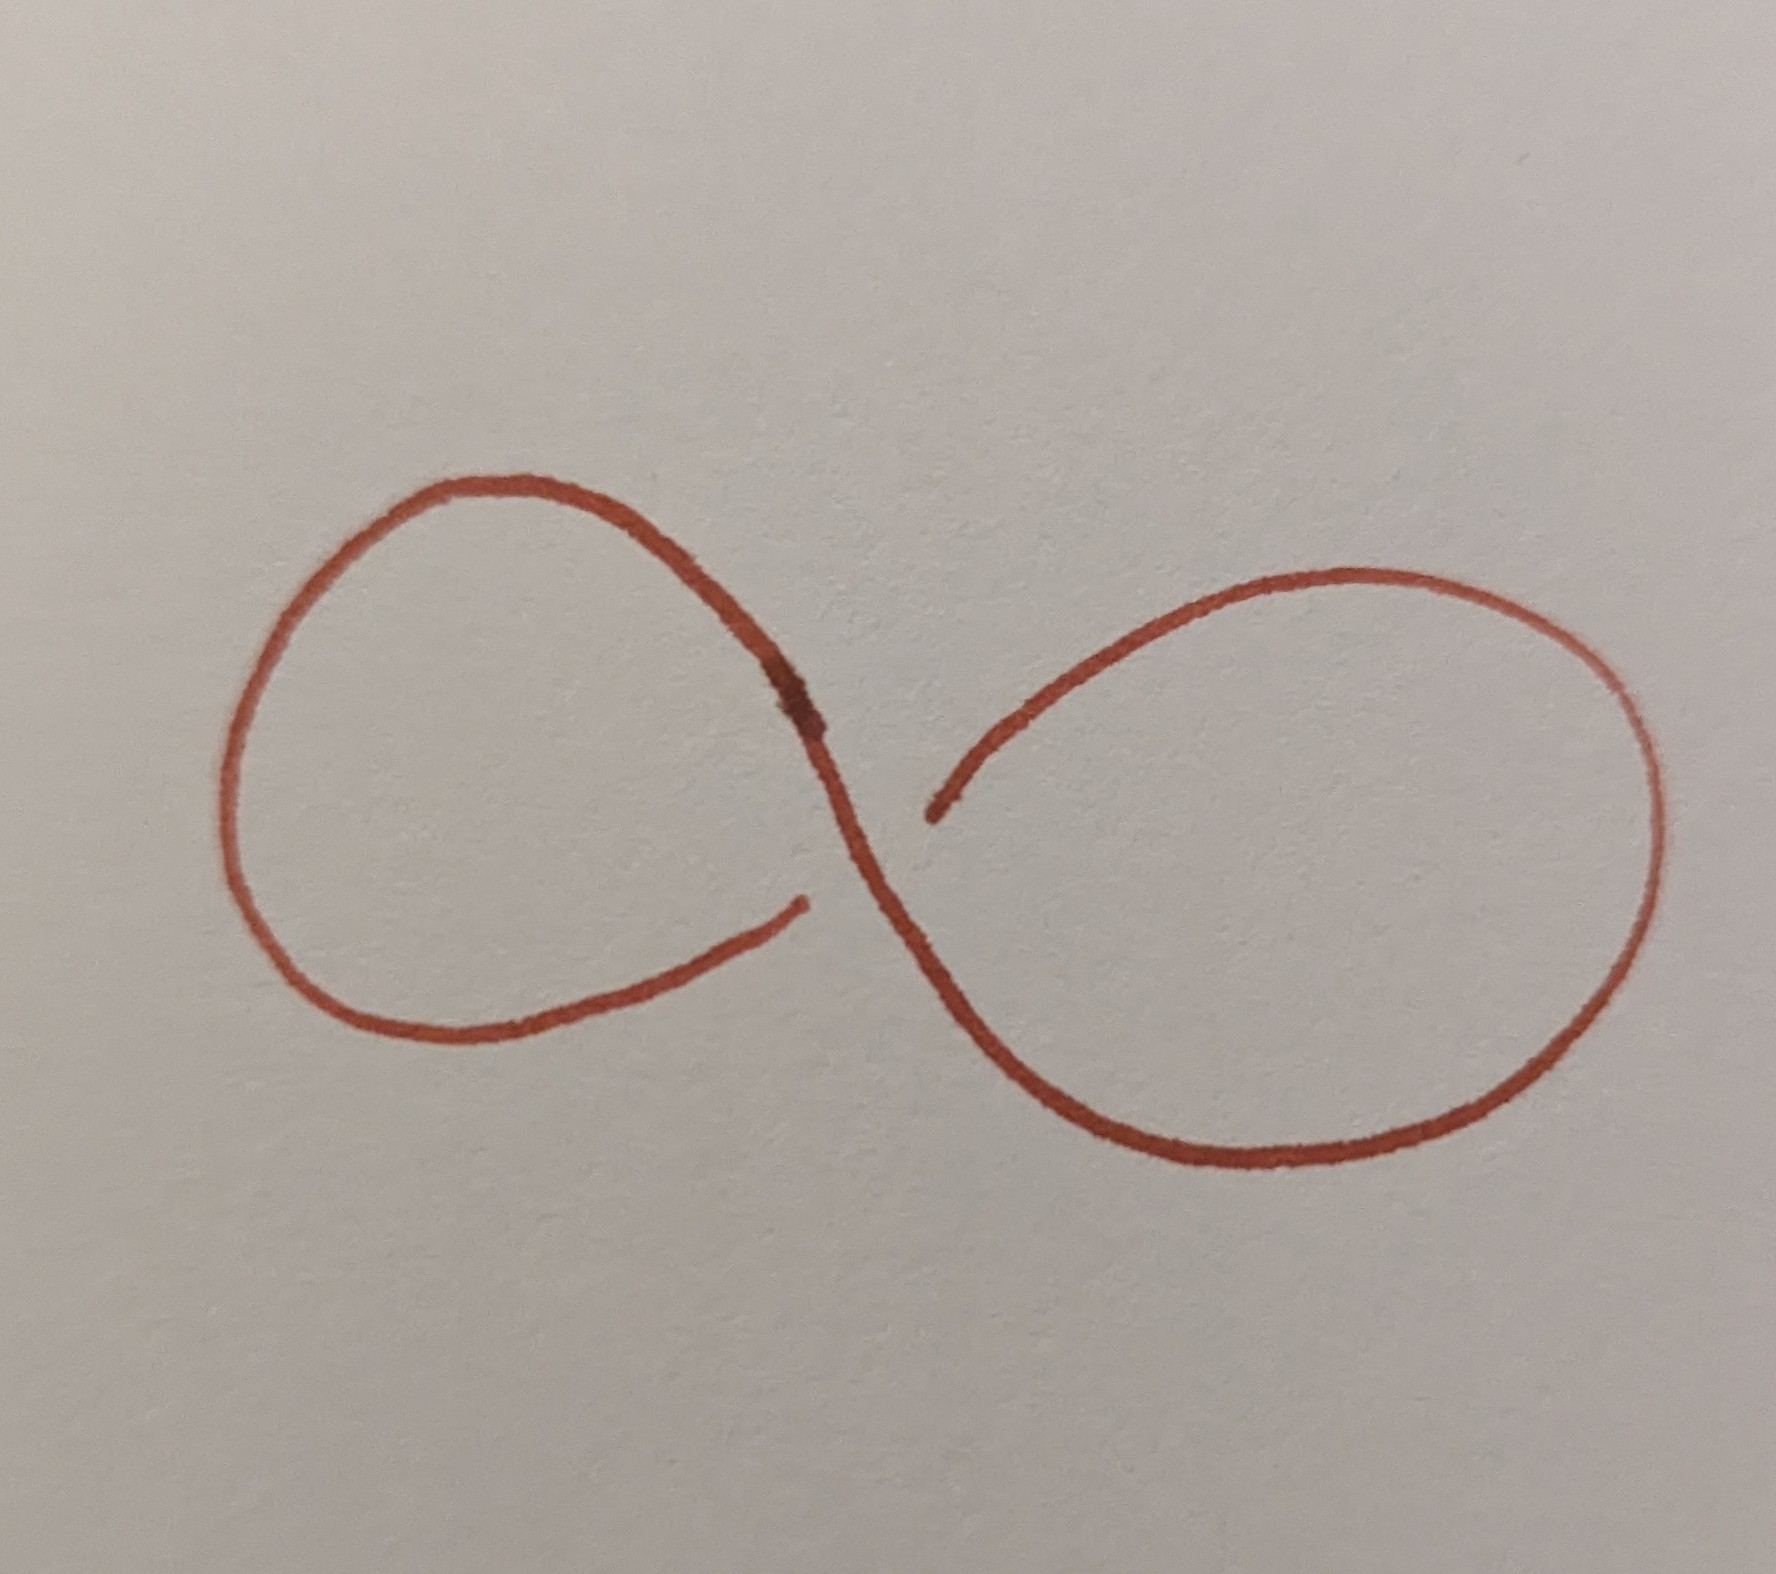
\includegraphics[width=0.25\linewidth]{graphics/unknot_twisted}
	\caption{Also the unknot}
	\label{fig:unknot_twisted}
\end{figure}

Though the central objective of knot theory it to classify knots up to ambient isotopy, as one might imagine, it can be very hard to write down explicit ambient isotopies directly, and in practice we find ourselves using other tools to get the job done. Though it was claimed that the objects in Fig. \ref{knot-examples} were knots, they are really projections of knots onto the plane with markings we call \textit{crossings} to make clear that some \textit{strand} of the knot has gone over another strand when we would have otherwise lost that information in the projection. One might call this distinction pedantry, but it does precisely introduce the distinction between knots and the \textit{knot diagrams} given in Fig. \ref{knot-examples}. There are many diagrams for the same knot, in fact infinitely many. For brevity we may say `knot' when we should more strictly have said `knot diagram', but if it is not clear from context, we shall be precise.

Diagrams are much easier to work with than embeddings, and we have the following foundational theorem due to Kurt Reidemeister.
\begin{theorem}(The Reidemeister Theorem)
Two knot diagrams $D_{1}$ and $D_{2}$ represent equivalent knots if and only if there is some sequence of moves of the following four types that transform $D_{1}$ into $D_{2}$:
\begin{enumerate}[(1)]
	\item \notered{RI (insert image)},
	\item \notered{RII},
	\item \notered{RIII},
	\item planar isotopy.
\end{enumerate}
\end{theorem}

The early study of knot theory by pioneers such as P.G. Tait, C.N. Little and T. Kirkman involved trying to find, by hand, some way to show two knots were equivalent. But Tait himself noted that is was impossible by these means to ever prove that two knots were distinct. The modern way that we deal with knots is through invariants. If we define some map from knots to some other class of objects, perhaps a truth value, an polynomial, or a group, and can show that none of the Reidemeister moves, not planar isotopy changes the value of this map, then we have a \textit{knot invariant}. Finally we have a way to prove that two knots are different, for if they take on different invariants there can't be a way to get between them with the invariant-preserving Reidemeister moves, so by Reidemeister's theorem, they must be distinct. However invariants are one-sided in nature -- having different invariants can tell us that two knots are different, but two knots talking on the same value of some invariant doesn't necessitate that they be equivalent knots. Such an invariant would be called a \textit{complete} invariant, and while we now know of a whole zoo of different invariants, we have yet to find what is perhaps the Holy Grail of knot theory: a complete invariant that is also easy to compute.

\section{Alternating Knots, Knot Mutation and the Tait Graphs}
We call a knot diagram \textit{alternating} if, traversing the diagram, the crossings alternate under and over. Clearly, for every diagram that is alternating, it is possible to construct a non-alternating diagram of an equivalent knot, simply apply one instance of RI. Hence we define an \textit{alternating knot} as a knot that has some alternating diagram. \notered{Alternating knots are interesting. Possibility to talk about the Tait conjectures here. Need at least the following.} Any two equivalent alternating knots is related by a sequence of flype moves. \notered{Expand on this including find the reference to a proof of the flyping theorem.}

We also have ways of constructing new knots from existing ones. A \textit{tangle} in a knot diagram is a region of the plane, surrounded by a circle such that the knot crosses that circle exactly four times. If we take a diagram, choose a tangle, and then perform some reflection (up to planar isotopy) of that tangle, either reflecting it left-right or up-down, or across one of the diagonals, the corresponding operation on the knot is known as \textit{mutation}, and the two knots known as mutants. Mutants are some of the hardest knots to distinguish in knot theory, as a number of the key invariants are the same on mutants. An example of this is the Conway Knot and the Kinoshita-Terasaka knot (Fig. \ref{fig:kinoshita-terasaka-mutants}).

\begin{figure}[h]
	\centering
	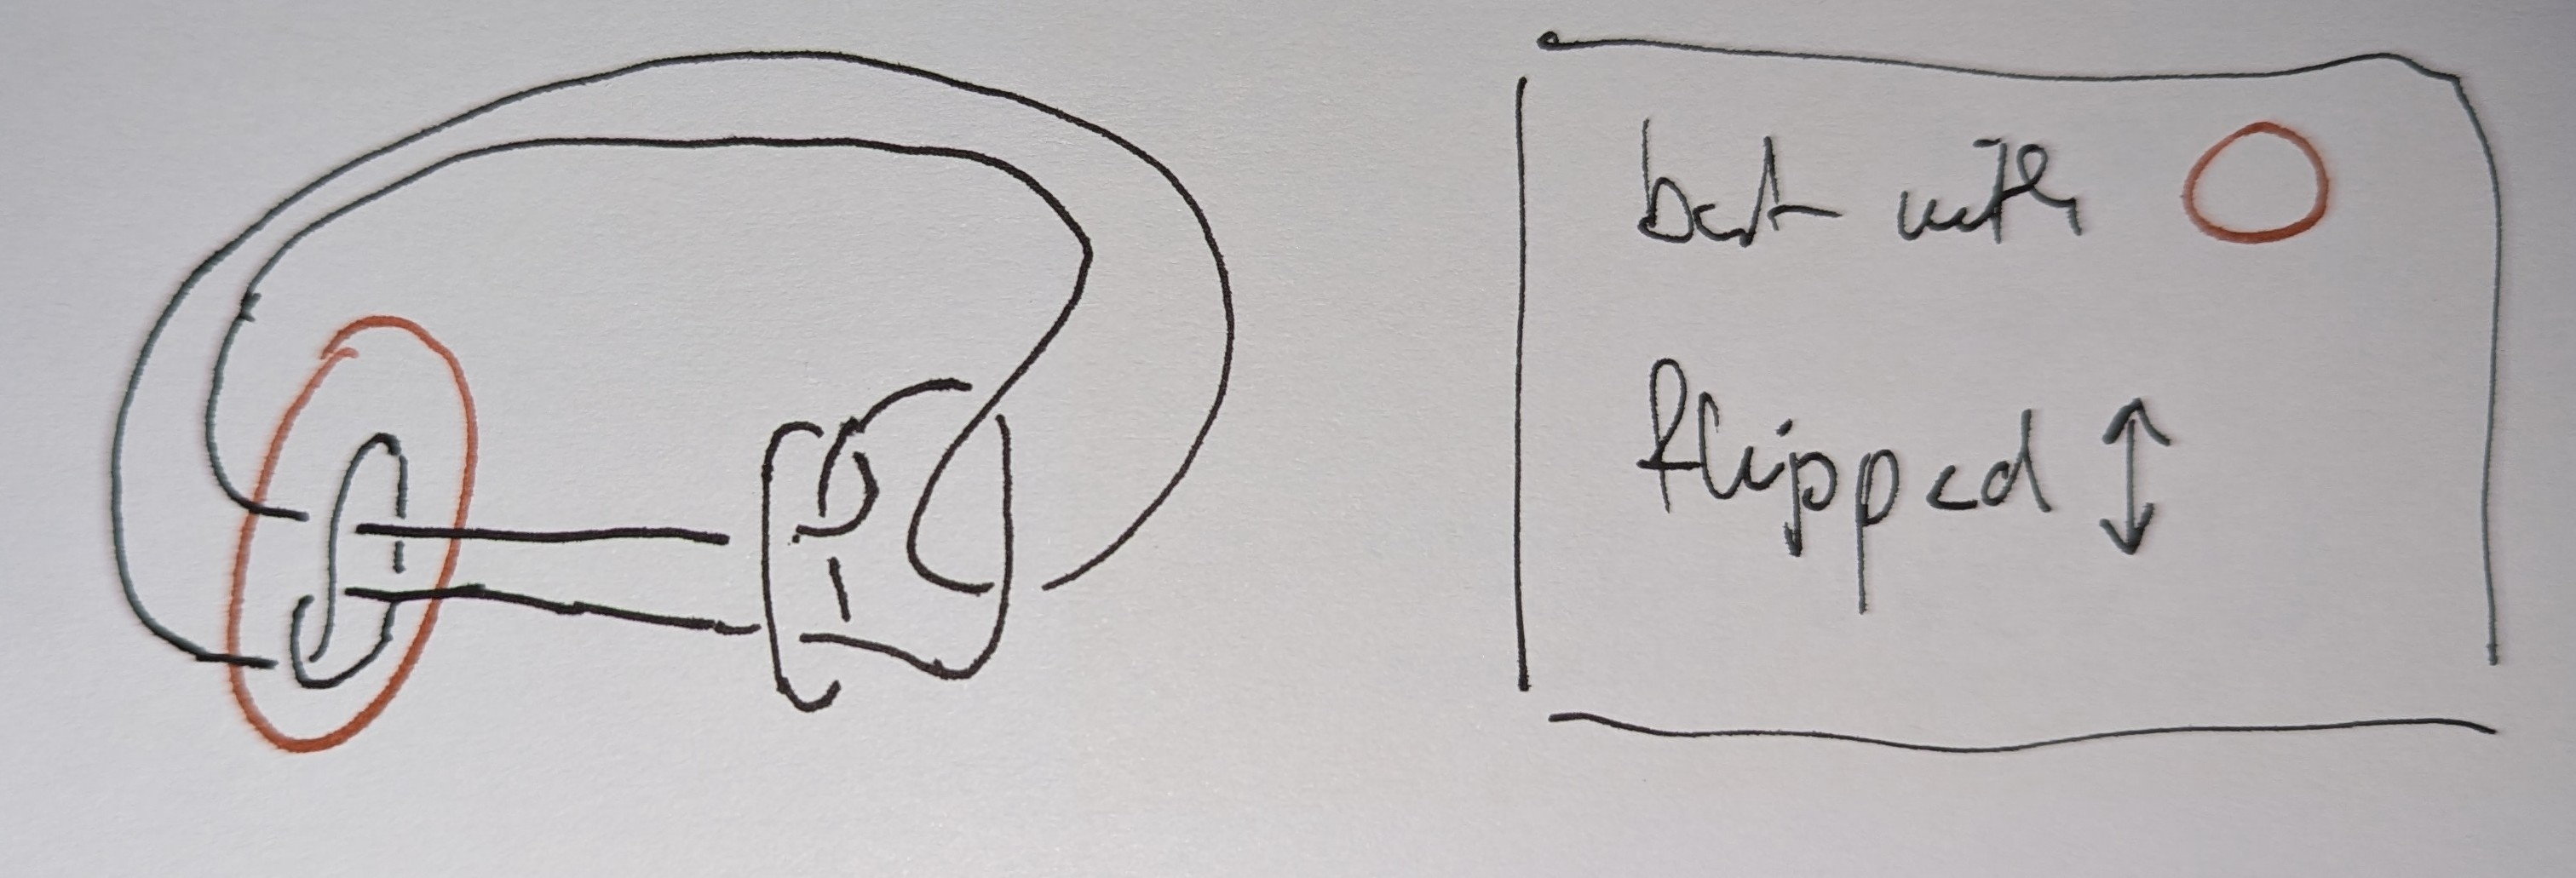
\includegraphics[width=0.95\linewidth]{graphics/Kinoshita_Terasaka_mutants}
	\caption{The Kinoshita-Terasaka knot and the Conway knot, an example of two mutants. \notered{Check which one is which!}}
	\label{fig:kinoshita-terasaka-mutants}
\end{figure}

For every knot diagram, we can associate a pair of graphs known as the \textit{Tait graphs}. We take the knot diagram, which divides the plane into regions. It is an application of the Jordan curve theorem that it is possible to colour these regions two colours, black and white, such that adjacent regions are never the same colour. Such a colouring is called a \textit{checkerboard colouring}. In such a colouring, regions that are diagonal to each other at crossings are necessarily the same colour. One Tait graph corresponds to the black colouring and has vertices inside each black region, and for each crossing, an edge connecting black regions diagonal to each other at that crossing. Similarly, another Tait graph, the planar dual of the first, can be constructed replacing with the white regions. \notegreen{Red and green regions may work better for diagrams.} \notered{Add figures.}


\section{The Lattice of Integer Flows}

For the rest of this chapter, we largely follow the work of \cite{lattices-graphs-mutation} to introduce the lattice of integer flows and show that it is a complete mutation invariant of alternating knots. This means that it is both an invariant of virtual knots, and among virtual knots, it takes on equivalent values on exactly those virtual knots that are of the same mutation class. We then talk about the equivalent formulation given in \cite{lattices-graphs-mutation} as the $d$-invariant.

A \textit{lattice} is a finitely generated abelian group $L$, equipped with an inner product 
\({\ip{\cdot}{\cdot}: L \times L \longrightarrow \R}\). We are primarily interested in \textit{integral lattices}, for which the inner product's image is contained within $\Z$, and for the rest of this text we assume that all lattices are integral. An \textit{isomorphism of lattices} is a bijection $\psi: L_{1} \longrightarrow L_{2}$ that preserves the inner product, that is ${\ip{x}{y} = \ip{\psi(x)}{\psi(y)}}$ for all $x, y \in L$.

Throughout, we let $G = (E, V)$ be a finite, directed, connected graph (in which loops and multiple edges are allowed) with vertex set $V$ and edge set $E$. The boundary map $\partial:  C_{0}(G) \longrightarrow C_{1}(G)$ defines a $|V|\times|E|$ incidence matrix $D : \Z^{E} \longrightarrow \Z^{V}$ with entries given by
\[D_{ij} = \begin{cases}
	+1 & \text{if $e_{i}$ is oriented into $v_{j}$}   \\
	-1 & \text{if $e_{i}$ is oriented out of $v_{j}$} \\
	0  & \text{otherwise.}
\end{cases}\]

The \textit{lattice of integer flows} of $G$ is the group $\Lambda(G) = \ker D$, along with the inner product induced by the Euclidean inner product on $\Z^{E}$. Equivalently, $\Lambda(G)$ is the first homology group of $G$, with inner products taken in $C_{1}(G)$. While the lattice $\Lambda(G)$ may depend on the orientation of the edges in $G$, its isomorphism class does not, as the isomorphism class of the homology group is independent of orientation, and the Euclidean inner product is preserved by sending an edge to its negation, since in the Euclidean inner product, $\ip{e_{i}}{e_{i}} =  \ip{-e_{i}}{-e_{i}} = 1$, and $\ip{e_{i}}{e_{j}} = \ip{-e_{i}}{e_{j}} = 0$.

\notegreen{TODO: Perhaps put an example of a lattice of integer flows?}

A \textit{$2$-isomorphism} between two graphs $G = (E, V)$ and $G' = (E', V')$ is a bijection \({\psi: E \longrightarrow E'}\) that preserves cycles, i.e. $\partial(e_{i} + \cdots + e_{j}) = 0$ if and only if $\partial\left(\psi(e_{i}) + \cdots + \psi(e_{j})\right) = 0$. We call and edge $e$ of a graph $G$ a \textit{bridge} if the removal of $G$ from $e$ disconnects $G$, and we say a graph $G$ is \textit{$2$-edge-connected} if $G$ has no bridges.

It is well established that of $2$-edge-connected graphs, $2$-isomorphism implies isomorphic lattices of integer flows; that is $\Lambda(G)$ is a $2$-isomorphism invariant of $2$-edge-connected graphs \parencite{lattice-of-flows-cuts}. More interestingly, and more recently, due to Su-Wagner \cite[Theorem 1]{lattice-of-flows-regular-matroid} and Caporaso-Viviani \cite[Theorem 3.1.1]{torelli-for-graphs-tropical-curves}, the converse is also true.


\begin{theorem}
For two $2$-edge-connected graphs $G$ and $G'$, $\Lambda(G) \cong \Lambda(G')$ if and only if $G$ and $G'$ are $2$-isomorphic. That is, $\Lambda(G)$ is a complete $2$-isomorphism invariant of $2$-edge-connected graphs.
\end{theorem} $\Lambda(G) \cong \Lambda(G')$ if and only if $G \simeq^{2} G'$, that is, the lattice isomorphism class of $\Lambda(G)$ is a complete $2$-isomorphism invariant of graphs.

Two graphs $G$ and $G'$ are related by a \textit{Whitney flip} if it is possible to find two disjoint graphs $\Gamma_{1}$, with distinguished vertices $u_{1}$ and $v_{1}$ and $\Gamma_{2}$ with distinguished vertices $u_{2}$ and $v_{2}$, such that the identifications $u_{1} = u_{2} = u$ and $v_{1} = v_{2} = v$ form $G$, and the identifications $u_{1} = v_{2} = u'$ and $v_{1} = u_{2} = v'$ form $G'$. An example of graphs related by a Whitney flip is given in Fig. \ref{fig:whitney_flip}.

\begin{figure}[hbt]
	\centering
	\def\svgscale{0.5}
	\input{graphics/whitney_flip.pdf_tex}
	
	\caption{An example of a Whitney flip.}
	\label{fig:whitney_flip}
\end{figure}

It is clear that sequences of Whitney flips only ever transform graphs within their $2$-isomorphism class, as cycles map to cycles. From \cite{2-isomorphic-graphs}, we have the important converse; a Reidemeister-like theorem for $2$-isomorphic graphs.

\begin{theorem}[Whitney's Theorem]
Two graphs $G$ and $G'$ are $2$-isomorphic if-and-only-if there is a sequence of Whitney flips relating $G$ to $G'$.
\end{theorem}

It can be easily shown that flype moves correspond to Whitney flips of the Tait graphs of the knot. Since all Tait graphs of reduced alternating knots are $2$-edge-connected, it is an immediate consequence of Whitney's theorem is that that pair $\Lambda(G_{1}), \Lambda(G_{2})$, where $G_{1}$ and $G_{2}$ are the Tait graphs of the knot is an invariant of alternating knots.

Greene proves that a mutation of alternating knot diagrams induces at worst a Whitney flip on the the Tait graph, and and a Whitney flip on the Tait graph induces a mutation on the diagram. This completes the proof of the following theorem (Proposition 4.4 in \cite{lattices-graphs-mutation}).

\begin{theorem}[Greene]
For a knot $K$, the pair $\Lambda(G_{1}), \Lambda(G_{2})$ of lattices of integer flows of the Tait graphs, which we denote as $\Lambda(K)$ is an complete mutation invariant of alternating knots. That is,
\begin{enumerate}[(1)]
\item $\Lambda(K)$ is an invariant of alternating knots, and
\item Alternating knots $A_{1}$ and $A_{2}$ are mutants if and only if $\Lambda(A_{1}) \cong \Lambda(A_{2})$.
\end{enumerate}
\notered{Give some notes about what it means to have an `isomorphism of the pair' $\Lambda(G_{1}), \Lambda(G_{2})$ for $G_{1}$, $G_{2}$ Tait graphs of $D$.}

\end{theorem}

\section{\notegreen{The $d$-invariant and Heegard-Floer Homology}}
\notegreen{Show that can be compressed into the $d$-invariant, and nothing is lost.}

\chapter{Virtual Knots}

\chapter{Gordon-Litherland Linking Form}

\chapter{Gauss Codes and Knot Algorithms}
\notered{Work in pages already written about the algorithm to find the Tait graph.}


\chapter{Computing Mock Seifert Matrices}


\chapter*{Acknowledgements}
\addcontentsline{toc}{chapter}{Acknowledgements}

Thanks to ...

\newpage
\printbibliography[title=References]


\appendix
\titleformat{\chapter}[block]
  {\normalfont\Large\bfseries}{Appendix \thechapter}{1em}{\Large}
\titlespacing*{\chapter}{0pt}{40pt}{30pt}

\chapter{Algorithm}


\end{document}

